\section{Modernização de Software}\label{ms}

A condução de mapeamento sistemático (MS) na área de 
Engenharia de Software tem se tornado uma prática 
consolidada que envolve um conjunto bem definido 
de atividades~\cite{Petersen:2008}. Esta seção descreve 
o resultado da primeira análise realizada no MS com o intuito de caracterizar a modernização dos sistemas legados no contexto da manutenção de software, ao identificar 
as principais contribuições e estudos na literatura sobre este tema. Mais detalhes deste estudo foram submetidos ao \textit{The 31st ACM/SIGAPP Symposium on Applied Computing} (ACM SAC 2016). Para tal estudo, um protocolo de estudo foi elaborado, de modo a permitir sua reprodução por outros pesquisadores, sem os problemas do viés de publicação mencionados em~\cite{kitchenham:2004}.

\subsection{An\'{a}lise Relacionada à Primeira Questão de Pesquisa}

A modernização pode ser caracterizada, de acordo com~\cite{S01_bennett2000software, S9_bianchi:2003, S3_Bisbal:1999, S15_Comella-DordaASurvey2000, S2_erlikh:2000}, pela necessidade de evolução dos sistemas para adequá-lo aos requisitos de negócio das organizações, seja com novas funcionalidades, correção de erros ou atualizações tecnológicas. Nesse sentido, muitas teorias tem sido sugeridas na literatura, como discutido a seguir. 

\textbf{N. Weiderman et al.} introduzem um modelo de ciclo de vida 
para descrever a evolução de um sistema durante a sua vida útil~\cite{S15_Comella-DordaASurvey2000, Seacord:2003, S12_WeidermanApproaches:1997}. 
Neste modelo, existem três fases distintas: manutenção, modernização e substituição.  Nesse ciclo, as necessidades de negócio da organização são intercaladas com as implementações realizadas para suprir essas necessidades. 
Além de introduzir um modelo de ciclo de vida, Weiderman et al. também propõem distinguir a modernização pelo nível de compreensão requerido para suportar 
os esforços de modernização: \textit{White-box} para compreensão das estruturas internas do sistemas e \textit{Black-box} quando requer a compreensão das interfaces externas dos sistemas legados.

\textbf{K. Bennett et al.} propõem um modelo chamado 
\textit{staged model} para descrever o ciclo de vida de um sistema e auxiliar na identificação das principais 
áreas de pesquisa sobre modernização~\cite{S01_bennett2000software}. Este modelo divide-se em 5 etapas: 
\textit{initial development, evolution, servicing, phase-out, close-down}. Aqui, a modernização compreende a fase \textit{evolution} e, 
ao contrário do modelo proposto por Weiderman et al., é considerada uma atividade de manutenção, que pode ser classificada em 
4 classes: adaptativa, quando há alterações no ambiente do software; perfectiva, para novos requerimentos do usuário; corretiva, correção de erros; e preventiva, para 
prevenir problemas futuros. 

\textbf{J. Bisbal et al.} apresentam um modelo de ciclo de vida, onde o foco são as atividades evolutivas ordenadas pelo impacto causado nos 
sistemas~\cite{S3_Bisbal:1999}. Assim, dividem-se em \textit{wrapping}, cujo objetivo é prover uma nova interface para os componentes de um sistema, 
tornando-os mais acessíveis para outros componentes; manutenção, para os pequenos ajustes e correção de erros; a migração, que visa mover o sistema 
legado para um ambiente mais flexível, mantendo os dados e funcionalidades originais; e o redesenvolvimento, que reescreve por completo as aplicações. 

Percebe-se que, embora esses modelos usem termos distintos para referir-se as fases do ciclo de vida dos sistemas, há várias semelhanças. Por exemplo, 
o significado de substituição ~\cite{S15_Comella-DordaASurvey2000, Seacord:2003, S12_WeidermanApproaches:1997} é o mesmo que redesenvolvimento ~\cite{S3_Bisbal:1999} e o significado de migração ~\cite{S3_Bisbal:1999} é o mesmo que modernização ~\cite{S15_Comella-DordaASurvey2000, Seacord:2003, S12_WeidermanApproaches:1997}. No entanto, 
a fase \textit{wrapping} descrita por Bisbal et al. é uma técnica de modernização \textit{Black-box} em Weiderman et al. ~\cite{S15_Comella-DordaASurvey2000, Seacord:2003, S12_WeidermanApproaches:1997}.

Com a caracterização da modernização de software, finaliza-se esta análise com um \textit{word cloud}, disponível na figura ~\ref{fig:word_cloud}, dos 30 termos mais citados nos \textit{abstracts} das fontes primárias selecionadas para o MS. Note que, sob a perspectiva tecnol\'{o}gica, \'{e} poss\'{i}vel perceber nessa figura um certo grau de interesse na computa\c c\~{a}o orientada a servi\c cos. 


\begin{figure}
\centering
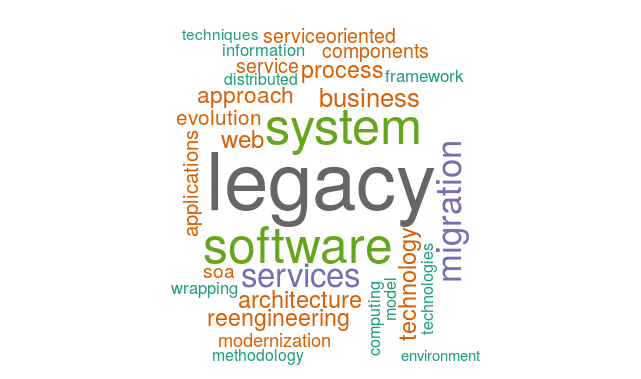
\includegraphics[scale=0.5]{figuras/word_cloud.png}
\caption{Termos mais citados nas publicações selecionadas}
\label{fig:word_cloud}
\end{figure}
